\chapter{Results exploitation}
\label{cha:resultsexploit}

\begin{summary}
In this chapter, we show how the obtained results with multi-objective optimization can be used to help a designer, using multi-criteria decision aid. We present how the solutions can be analysed, with a multi-criteria point of view. Then we discuss on their possible actual use and how difficult it is to make the industry adopt it. We then propose some hints to make it integrated into design flows as we do believe that a multi-criteria paradigm can help in design integrated circuits and that it can progressively be of use since designers will have to face greater and greater challenges.
\end{summary}

Associated publications:
\begin{itemize}
\item N.A.V. Doan, D. Milojevic, F. Robert, Y. De Smet, "Using the PROMETHEE methodology for the design of 3D-stacked integrated circuits", \textit{1st International MCDA Workshop on PROMETHEE (IMW2014)}, Bruxelles (Belgique), January 2014
\item K. Lidouh, N.A.V. Doan, Y. De Smet, "PROMETHEE-compatible presentations of multicriteria evaluation tables", \textit{International Journal of Multicriteria Decision Making}, to be published (minor revision)
\item K. Lidouh, N.A.V Doan, Y. De Smet, "PROMETHEE-compatible presentations of multicriteria evaluation tables", \textit{2nd International MCDA Workshop on PROMETHEE (IMW2015)}, Bruxelles (Belgique), January 2015, to be published (accepted)
\end{itemize}

\section{Introduction}
In Chapter \ref{cha:model} we have defined the problem we are dealing with in this work, show how a 3D-SIC can be modelled, as well as simulation results based on multi-objective optimization. In Section \ref{sec:robustness}, we have shown that the methodology can show good convergence and diversity properties even if the problem contains criteria of heterogeneous nature. In this chapter, we will discuss about how a designer could use these results and take advantage of a multi-criteria oriented methodology in the process of producing a 3D-SIC to, for instance, make a choice among the solutions of the Pareto frontier.

As explained in Chapter \ref{cha:rol.mcda}, once a Pareto front has been determined or approximated, the next step is to choose among this set of solutions. The simulations performed in the experiments of Section \ref{sec:robustness} have produced 804 individuals in the Pareto front and with such a large number of alternatives, choosing is not always trivial.

\section{Preference modelling}
One way to help decision makers to make their choice is to model their preferences, for instance with an outranking method. In the scope of this work, we will present the use of the PROMETHEE methodology as it has been developed in our department with an efficient software called D-Sight and has also shown good results in different fields \cite{Beh2010}. In addition, using this method can be justified as the evaluations are quantified. Also, even if the number of alternatives is large, PROMETHEE does not require a large number of inputs from the decision maker, as opposed to some other methods such as AHP (see Chapter \ref{cha:rol.mcda}) where pairwise comparisons of alternatives can be asked to a DM.

\subsection{Using the PROMETHEE methods}

\subsubsection{Building a PROMETHEE model}
In order to use the PROMETHEE method, the decision maker has to inform about his preferences on the criteria, these being preference functions, indifference and preference thresholds and weights on the criteria (see Chapter \ref{cha:rol.mcda}). To illustrate this, we will use a PROMETHEE software called D-Sight that has been developed by Quantin Hayez and use the results of the simulations presented in Section \ref{sec:robustness}. In those results, there are 804 alternatives in the Pareto front, evaluated on 5 criteria. The evaluation table can be found in Appendix \ref{apdx:prom804}. Let us take a simple example of preference modelling in order to illustrate what kind of aid a multi-criteria analysis can provide.

First, we have to define preference functions for each criterion. For the interconnection distance, cost, volume and clock position, we will choose a V-shape function. For these criteria, using this function, the preference index will increase linearly until a preference threshold is reached. For the power dissipation, we will choose a U-shape function where there is no preference until an indifference threshold is reached. Indeed there can be no real problem if the difference between two circuits in terms of heat dissipation is low, and it can be directly problematic when this difference is high.

The thresholds will be set at a difference of 10\% in the evaluations. For the weights, we will consider that the interconnection distance, the cost and the power dissipation are more important than the volume and the clock position, with the volume less important than the clock position. We will choose the weights by considering that the three first cited criteria share the same importance, 25\% each, and the two remaining ones taking the last 25\% (14\% and 11\% respectively). The robustness of this set of weights can be studied with a sensitivity analysis that will allow to confirm whether or not the variability of a weight will change the ranking. Let us note that it is possible to elicit the weights by answering simple questions, for instance with AHP.

A summary of all these data is given in Table \ref{tab:preffunc}. Of course, a more accurate model could be defined, however let us remind that the purpose here is to show how a multi-criteria analysis can give added information to designers.

\begin{table}[h!]
\caption{PROMETHEE model}
\begin{center}
\begin{tabular}{|c|c|c|c|c|}
\hline
Criterion & Preference & Indifference  & Preference & Weight \\
 & function & threshold & threshold & \\
\hline
Interconnection distance & V-shape & x & 10\% & 25\% \\
Cost & V-shape & x & 10\% & 25\% \\
Volume & V-shape & x & 10\% & 11\% \\
Clock position & V-shape & x & 10\% & 14\% \\
Power dissipation & U-shape & 10\% & x & 25\% \\
\hline
\end{tabular}
\end{center}
\label{tab:preffunc}
\end{table}

Now that a model has been proposed, let us analyse the results produced by D-Sight.

\subsubsection{Multi-criteria analysis}

\paragraph{PROMETHEE rankings}
D-Sight will do all the computations of the flows and PROMETHEE (I and II) rankings can be obtained, based on the preferences. A decision maker can make a choice based on these rankings, for example by choosing the solution ranked first. In addition, other tools are available, that allow to have a transparent decision process and analyse the set of solutions to know why a given ranking is obtained. One of the most useful one is the GAIA plane which is illustrated in Figure \ref{fig:gva804} (for the sake of readability, the alternative names have been removed).

\begin{figure}[h!]
\begin{center}
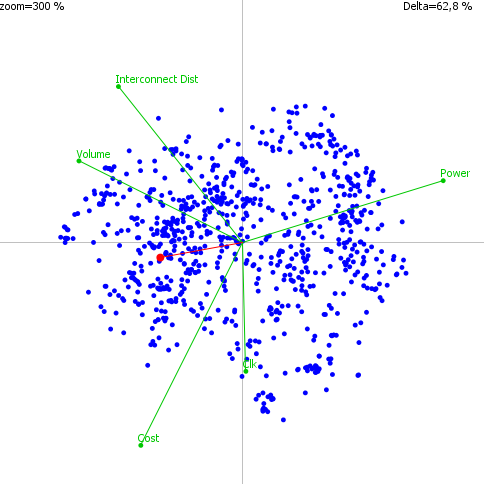
\includegraphics[width=0.8\linewidth]{gva804}
\end{center}
\caption{GAIA plane of the case study}
\label{fig:gva804}
\end{figure}

As a reminder from Chapter \ref{cha:rol.mcda}, the GAIA plane is based on the principal component analysis of the unicriterion net flows of the solutions and minimises the projection error of each alternative on it. Four distinctive visual information are shown:
\begin{enumerate}
\item The green axes that represent the projections of each criterion's axis.
\item The blue dots that represent the projection of each solution's uni-criterion net flow. The value of the uni-criterion net flow is read by projecting the point on the related criterion axis.
\item The red axis that represents the \textit{decision axis} which is the projection of the set of weights and gives the decision direction.
\item The \textit{delta} value that represents the percentage of kept information since there are projection errors.
\end{enumerate}

The first observation that can be drawn is that the blue dots are at the same time well-spread and dense, which illustrate the conclusions of Section \ref{sec:robustness}. This also means that each criterion is well-represented in terms of solutions.

Second, let us take a look at the information that is provided by the criteria axes (green). This is shown in Figure \ref{fig:gva804crit}.

\begin{figure}[h!]
\begin{center}
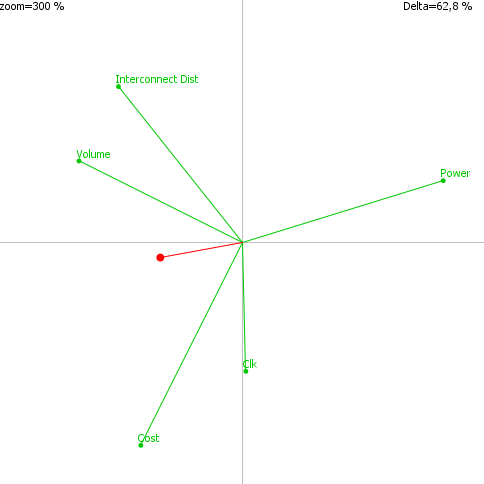
\includegraphics[width=0.8\linewidth]{gva804crit}
\end{center}
\caption{GAIA plane of the case study (criteria axis only)}
\label{fig:gva804crit}
\end{figure}

From the GAIA plane, we can observe how the criteria are related between each other. Indeed, criteria axes that have opposite directions are conflicting, whereas criteria with the same direction are in synergy. In the present case, we can see that the criteria of interconnection distance, power dissipation and cost are conflicting, which reflects the design reality. Also, the volume criterion shares the same direction as the interconnection distance criterion which is normal as reducing the interconnection distance will also tend to reduce the circuit volume. These observations also confirm that the defined model is indeed consistent with the reality.

Finally, let us have a view at the information provided by the decision axis. As explained previously, the decision axis represent the criteria weights and therefore gives the decision direction. Indeed, the alternatives with the highest net flow score will have their furthest projection on that axis, in the direction of that axis (see Figure \ref{fig:gva804stick}). This visually represents the PROMETHEE II ranking, provided that the \textit{delta} value shows that enough information has been kept with the projection. In this case, this value is relatively low (62.8\%) which means that a lot of information has been lost with the projection, that can lead, for instance, to PROMETHEE II ranking errors with the visual projections compared to the ranking obtained with the computed net flows.

\begin{figure}[h!]
\begin{center}
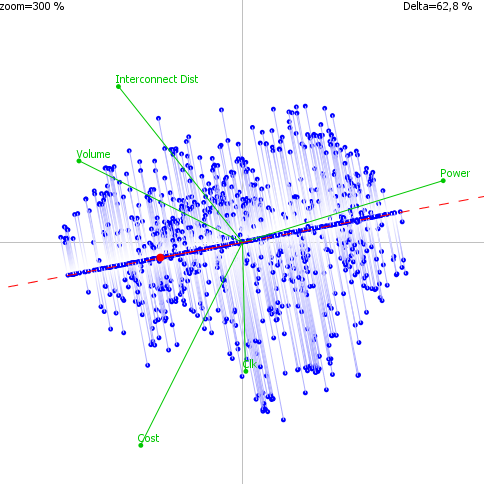
\includegraphics[width=0.8\linewidth]{gva804stick}
\end{center}
\caption{GAIA plane of the case study (with decision axis projection)}
\label{fig:gva804stick}
\end{figure}

\paragraph{Robustness analysis with stability intervals}
Another tool that can help decision makers is the robustness analysis that will allow them to know how stable a solution is, given the provided preference model. It is based on stability intervals on the weights where the first-ranked alternative will not change. This tool can be useful as there can be uncertainties on the values given for the weights. For the considered model, the stability intervals are shown in Table \ref{tab:stability}. We can observe that the first-ranked solution is relatively robust with all the criteria weights spanning on rather large intervals. This means that small uncertainties will not affect the ranking of the first alternative.

\begin{table}[h!]
\caption{Stability intervals (level 1)}
\begin{center}
\begin{tabular}{|c|c|c|c|}
\hline
Criterion & Min weight & Value  & Max weight \\
\hline
Interconnection distance & 5.73\% & 25\% & 50.00\% \\
Cost & 3.37\% & 25\% & 36.38\% \\
Volume & 0.00\% & 11\% & 23.85\% \\
Clock position & 2.06\% & 14\% & 43.06\% \\
Power dissipation & 17.85\% & 25\% & 68.21\% \\
\hline
\end{tabular}
\end{center}
\label{tab:stability}
\end{table}

As we can observe, the PROMETHEE methodology can help a decision maker facing choices and provide a transparent process. While the tools have been developed in order to be simple to use and analyse, the main difficulty is to model the preferences accordingly with a designer's needs. As the specifications required for a design cannot translate easily into preference information, establishing a preference model is not a trivial task and this will therefore need further investigations to adapt this methodology for designers.

\section{Constraint modelling}
To ease decision making, it is also possible to model constraints in order to eliminate unrequired alternatives and reduce the number of solutions, which will ease the choice process. For that purpose, we have developed a visual interface where a decision maker can introduce constraints to be fulfilled and see directly the remaining solutions that fit these requirements. The general interface is shown in Figure \ref{fig:dse1}.

\begin{figure}[h!]
\begin{center}
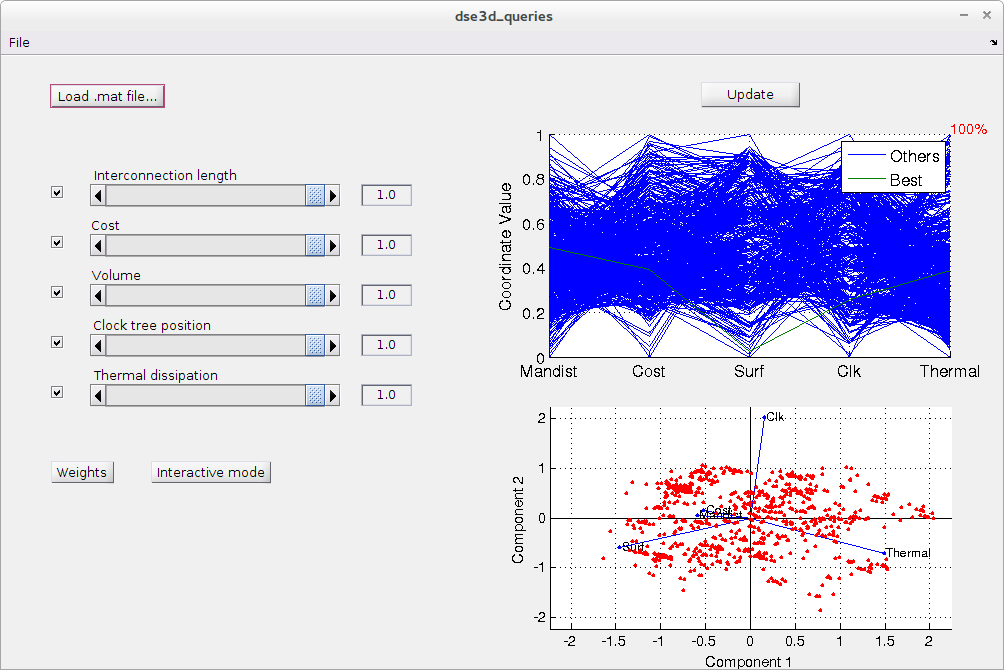
\includegraphics[width=\linewidth]{dseconstraints}
\end{center}
\caption{Constraints modelling (without filtered alternatives)}
\label{fig:dse1}
\end{figure}

The sliders are use to define the constraints. Two graphs are represented to visualise the solutions. The first one uses parallel axes. Let us note that, in order to use this representation effectively, we have normalised the evaluations between 0 and 1. The second graph is a PCA plane where the evaluations are projected (instead of the uni-criterion net flows for the GAIA plane). It can help a decision maker to more easily see in which direction the solutions are.

In Figure \ref{fig:dse2}, an example is shown where alternatives have been filtered. For illustration purposes, we have arbitrarily chosen values by considering normalized constraints of 0.5 for the interconnection length, 0.3 for the cost, 0.8 for the volume, 0.7 for the clock source position and 0.4 for the thermal dissipation (taking lower values means adding more constraints). Alternatives that do not reach these constraints are removed from the visualisation and we can see that from 804 potential solutions, there are 6 remaining possibilities which can ease the choice process.

\begin{figure}[h!]
\begin{center}
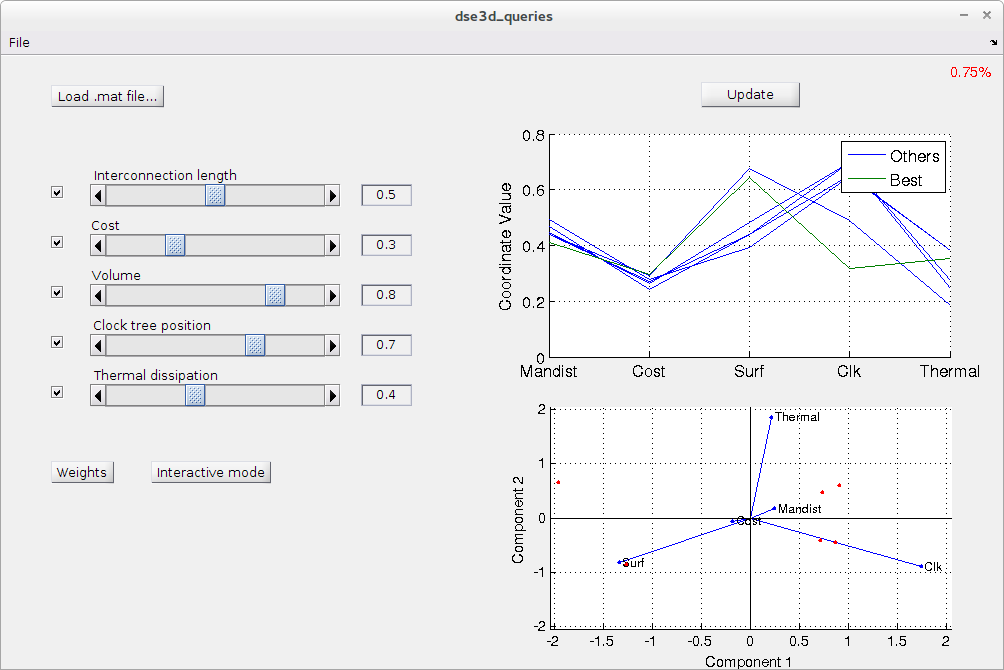
\includegraphics[width=\linewidth]{dseconstraints2}
\end{center}
\caption{Constraints modelling (with filtered alternatives)}
\label{fig:dse2}
\end{figure}

This software also allow the see the best profile given a set of weight for the criteria, by using a weighted sum. If these weights cannot be defined by the designer, they can be elicited with the AHP procedure that has been implemented within the interface.

This tool has been developed under Matlab and can be used for any problems that need to filter unrequired solutions with constraints to ease a decision process.

The users will eventually have to be aware that the evaluations have to be normalized between 0 and 1 in order to have an effective representation with the parallel axes. So, modelling the constraints can be more difficult than with the real evaluations. In the same way as preference modelling, the specifications cannot be easily translated into constraints so this would also require further investigations to adapt this method for designers.

\section{Pertinently representing multi-criteria information in evaluation tables}
Another way to help decision making could be to enrich evaluation tables with multi-criteria information. We have proposed a contribution with that purpose in \cite{LidDoaDes2014:techreport}. However, as it is difficult to find a direct application of this methodology in microelectronic design, this work will only be cited and reproduced in Appendix \ref{apdx:ijmcdm}.

\section{On the use of a multi-criteria paradigm in microelectronic design}
As described in Chapter \ref{cha:rol.icdesign}, the multi-criteria paradigm is rarely used in the field of IC design; at best, trade-off analyses are performed. To our knowledge, more global multi-criteria analyses have not been carried out yet.

When discussing with design experts, it is quite interesting to see how they easily understand the stake of the MCDA paradigm and how it would be able to help designers facing IC development challenges. However, it is more difficult to make them adopt this approach for three main reasons that have appeared throughout several discussions:

\begin{enumerate}
\item "It is not how we optimize circuits" seems to be one of the most frequent statements. Indeed, the industry follows a uni-criterion paradigm and is not used to first explore several possible solutions and then determine good compromise solutions. The designers will generally decide about an architecture and try to optimize it (following a uni-criterion paradigm) to fulfil the specifications.
\item Designers can understand how preference modelling work, however they are not used to answer questions about indifference/preference thresholds or criteria weights as they receive specifications to achieve. This would need a change in how the design of a circuit is approached and how specifications are formulated.
\item The design space exploration is based on performance estimation. While our model can provide consistent ordered information, the evaluations are not accurate. Therefore, modelling preference can be a more difficult task since it requires the designers to work with (assessed) values that are different from real specifications.
\end{enumerate}

As we can observe, the main reason of difficulties to adopt a multi-criteria paradigm lies in the lack of knowledge about this approach. This will need a deep work in all the steps in a design flow, from how the specifications are defined to the optimization processes. Specifications are currently more and more difficult to fulfil as the industry is nearing the limits of the present technologies. Changing how they are formulated, with therefore adequate methodologies, might help overcome this problem.

Also, (uni-criterion) optimization processes are nowadays more and more time-consuming (weeks to months). This can be seriously problematic in economical terms as a circuit will require more man-years. With this work, we have shown that applying a multi-objective optimization for design space exploration can shorten the design time. These simulations only last hours to days and can already give to designer assessments about the optimization of a circuit, which might lead to shorter optimization processes.

Finally, with the results we have obtained, we do believe that the multi-criteria analysis can aid designers when facing design challenges and allow them to make more transparent choices.

\section{Conclusion}
In this chapter, we have presented how the results of a multi-criteria approach can be exploited for designers. We have shown two ways to help in a decision process and cited a third work. Then we have discussed about the adoption of this paradigm in the field of microelectronic design where we have proposed some possible hints. Although the results we have obtained can provide relevant information to a designer that would not be available with current tools, their exploitation seems to be more complicated as it would require a change in how the industry works. Nevertheless, we do believe that a multi-criteria paradigm can help in design integrated circuits and that it can progressively be integrated into design flows since designers will have to face greater and greater challenges.